\documentclass[../cover.tex]{subfiles}

\begin{document}

\section{Tujuan}
    Tujuan dari praktikum ini sebagai berikut,
    \begin{enumerate}
        \item Mahasiswa dapat memahami mengenai state space.
        \item Mahasiswa dapat melakukan pemodelan sistem dalam bentuk state space.
        \item mahasiswa dapat memahami hubungan fungsi transfer dengan state space.
        \item Mahasiswa dapat menggunakan Matlab untuk mengkonversi suatu fungsi transfer kedalam bentuk state space maupun sebaliknya.
    \end{enumerate}
\section{Dasar Teori}
    Representasi \textit{state-space} merupakan persamaan yang terdiri atas dua bagian. bagian pertama merupakan persamaan \textit{state}. persamaan state merupakan set persamaan differensial orde satu dengan sejumlah \textit{state variables} n. Bagian kedua merupakan persamaan \textit{output} sistem, persamaan kedua merupakan kombinasi linier dari variabel \textit{state} dan variable \textit{input} suatu sistem\cite{Fahmizal}. persamaan umum dari representasi \textit{state-space} dinyatakan sebagai berikut,
\begin{equation}
    \begin{split}
        \dot{x} &= Ax+Bu \\[5pt]
              y &= Cx + Du
    \end{split}
\end{equation}
\section{Analisis}
    \subsection{Soal 1 Modul 1}
    Pada soal ini dilakukan analisis pada rangkaian RLC, mendapatkan persamaan fungsi alih serta mengkonversi persamaan tersebut menjadi persamaan \textit{state-space}.
    \begin{figure}[H]
        \centering
        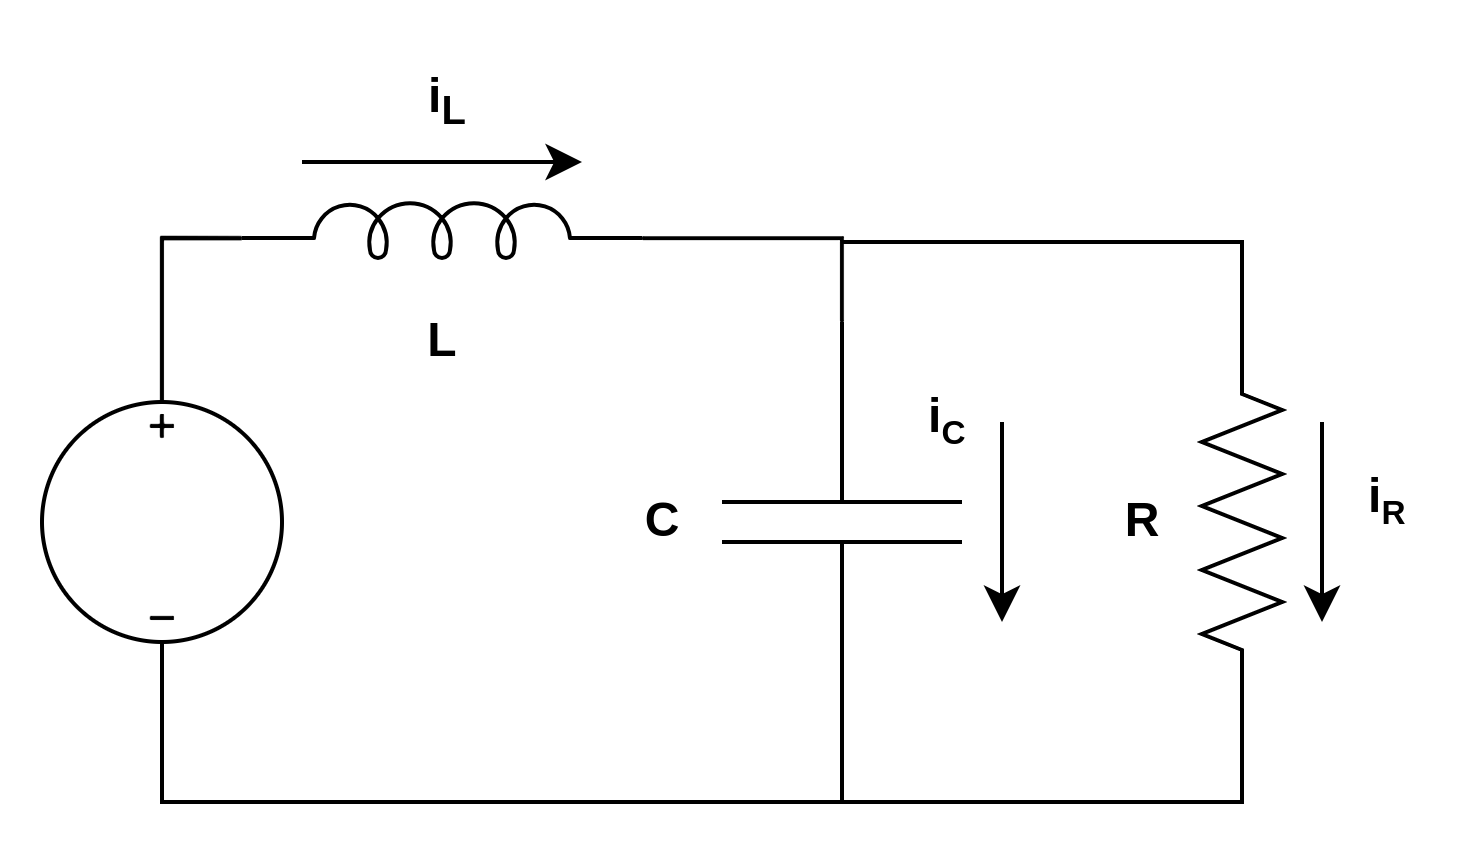
\includegraphics[width = 0.7\textwidth]{assets/image/rangkaianRLC.png}
        \caption{Rangkaian RLC}
        \label{gambar_6}
    \end{figure}
    Dari gambar rangkaian \ref{gambar_6} dapat digunakan hukum kirchoff arus dan hukum kirchoff tentang tegangan. Analisa untuk \textit{loop} satu sebagai berikut,
    \begin{equation}
        \begin{split}
                    V_{in} &= V_L + V_C \\[5pt]
                    V_{in} &= L\frac{di}{dt}+V_C \\[5pt]
            L\frac{di}{dt} &= V_{in} - V_C \\[5pt]
             \frac{di}{dt} &= \frac{1}{L} (V_{in} - V_C)
            \label{persamaan_23}
        \end{split}
    \end{equation}
    Analisa untuk \textit{loop} dua sebagai berikut,
    \begin{equation}
        \begin{split}
            I_L &= I_R + I_C \\[5pt]     
            I_R &= I_L - I_C \\[5pt]
        \end{split}
    \end{equation}
    Karena C dan R paralel maka $V_c = V_R$ sehingga,
    \begin{equation}
        \begin{split}
            \frac{V_R}{R} &= I_L - C\frac{dV_C}{dt} \\[5pt]
            \frac{V_C}{R} &= I_L - C\frac{dV_C}{dt} \\[5pt] \\[5pt]
            \frac{dV_C}{dt} &= \frac{1}{C} \left( I_L + \frac{V_C}{R} \right)
        \end{split}
    \end{equation}
    \subsection{Soal 2 Modul 1}
    Pada soal ini, dilakukan analisis untuk mengubah persamaan fungsi transfer menjadi persamaan \textit{state-space} sebagai berikut,
        \begin{equation}
            \begin{split}
                G_s &= \ffrac{4s+2}{2^2+14s+18} \\[5pt]
                \ffrac{y}{u} &= \ffrac{4s+2}{2s^2+14s+18} \\[5pt]
                \ffrac{y}{u} &= \underbrace{\frac{1}{2s^2+14s+18}}_\text{mencari $\dot{x}=Ax+Bu$} \overbrace{4s+2}^\text{mencari $y=Cx+Du$}
                \label{persamaan_1}
            \end{split}
        \end{equation}
        Dari Persamaan \eqref{persamaan_1} dapat dicari persamaan input state space sebagai berikut,
        \begin{equation}
            \begin{split}
                \frac{y}{u} &= \frac{1}{2s^2+14s+18} \\[5pt]
                1u &= (2s^2+14s+18)y \\[5pt]
                1u &= 2\frac{dy^2}{dt^2} + 14\frac{dy}{dt} + 18y \\[5pt]
                1u &= 2\ddot{y} + 14\dot{y} + 18y \\[5pt]
                \ddot{y} &= -7\dot{y}-9y+1u
                \label{persamaan_2}
            \end{split}
        \end{equation}
        Dari persamaan \eqref{persamaan_2} diperoleh aturan sebagai berikut,
        \begin{equation}
            \begin{split}
                x_1 &= y \\[5pt]
                x_2 &= \dot{x_1} = \dot{y}
                \label{persamaan_3}
            \end{split}
        \end{equation}
        Dari persamaan \eqref{persamaan_2} dan aturan \eqref{persamaan_3} dapat dicari persamaan \textit{input state-space} $\dot{x}=Ax+Bu$ sebagai berikut,
        \begin{equation}
            \begin{split}
                \dot{x}&=Ax+Bu \\[5pt]
                \begin{bmatrix} \dot{x_1} \\ \dot{x_2} \end{bmatrix} &= \begin{bmatrix} 0 & 1 \\ -9 & -7 \end{bmatrix} \begin{bmatrix} x_1 \\ x_2 \end{bmatrix} + \begin{bmatrix} 0 \\ 1 \end{bmatrix} u
            \label{persamaan_4}
            \end{split}
        \end{equation}
        persamaan \textit{output state-space} dapat dicari dengan menganalisa persamaan \eqref{persamaan_1} sebagai berikut,
        \begin{equation}
            \begin{split}
                \frac{y}{u} &= 4s^2 + 2 \\[5pt]
                y &= (4s+2)u \\[5pt]
                y &= 4\frac{du}{dt} + 2u \\[5pt]
                y &= 4\dot{u} + 2u
                \label{persamaan_5}
            \end{split}
        \end{equation}
        Pada persamaan \eqref{persamaan_2} yang merupakan bagian denumerator dibagi dengan dua sehingga bagian numerator yaitu persamaan \eqref{persamaan_5} juga dibagi dengan dua. Sehingga hasil akhirnya sebagai berikut,
        \begin{equation}
            y = 2\dot{u} + 1u
        \end{equation}
        berdasarkan peraturan \eqref{persamaan_3} dapat dideklarasikan bahwa,
        \begin{equation}
            \begin{split}
                x_1 &= u \\[5pt]
                x_2 &= \dot{x_1} = \dot{u}
                \label{persamaan_6}
            \end{split}
        \end{equation}
        persamaan \textit{output state-space} $y=Cx+Du$ dapat dicari dari persamaan \eqref{persamaan_5} dan aturan \eqref{persamaan_6} sebagai berikut,
        \begin{equation}
            \begin{split}
                y=\begin{bmatrix} 1 \hspace{5mm} & 2 \end{bmatrix} \begin{bmatrix} x_1 \\ x_2 \end{bmatrix}
                \label{persamaan_7}
            \end{split}
        \end{equation}
    Hasil analisa manual kemudian dibandingkan dengan analisa menggunakan MATLAB. Berikut merupakan kode program untuk konversi dari fungsi alih ke \textit{state-space},
    \begin{figure}[H]
        \centering
        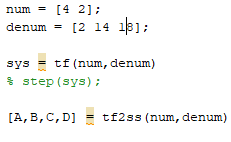
\includegraphics[width = 0.5\textwidth]{assets/image/kodeMatlab_.png}
        \caption{Kode program konversi fungsi alih ke persamaan \textit{state-space}}
        \label{gambar_7}
    \end{figure}
    Hasil dari program \ref{gambar_7} sebagai berikut
    \begin{figure}[H]
        \centering
        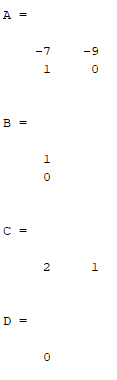
\includegraphics[width = 0.2\textwidth]{assets/image/outSSMatlab_.png}
        \caption{Hasil program konversi dari fungsi alih ke persamaan \textit{state-space}}
        \label{gambar_8}
    \end{figure}
    Dari hasil program MATLAB dapat dilihat bahwa hasil perhitungan secara manual sesuai dengan haasil dari program MATLAB. Posisi nilai-nilai pada matriks dari perhitungan manual dan program MATLAB berbeda karena urutan polynomial pada program MATLAB dimulai dari pangkat yang paling tinggi terlebih dahulu. Sedangkan, hasil perhitungan manual menempatkan pangkat polynomial yang kecil terlebih dahulu dalam urutan penulisannya.
    \subsection{Latihan Soal 1}
        \subsubsection{Menyederhanakan blok diagram}
        Terdapat diagram blok sistem sebagaimana ditunjukkan pada gambar \ref{gambar_1}, penyederhanaan blok dapat dilakukan dengan mengalikan $G_c$ dan $G_p$ sehingga didapatkan nilai untuk blok $G$.
            \begin{figure}[H]
                \centering
                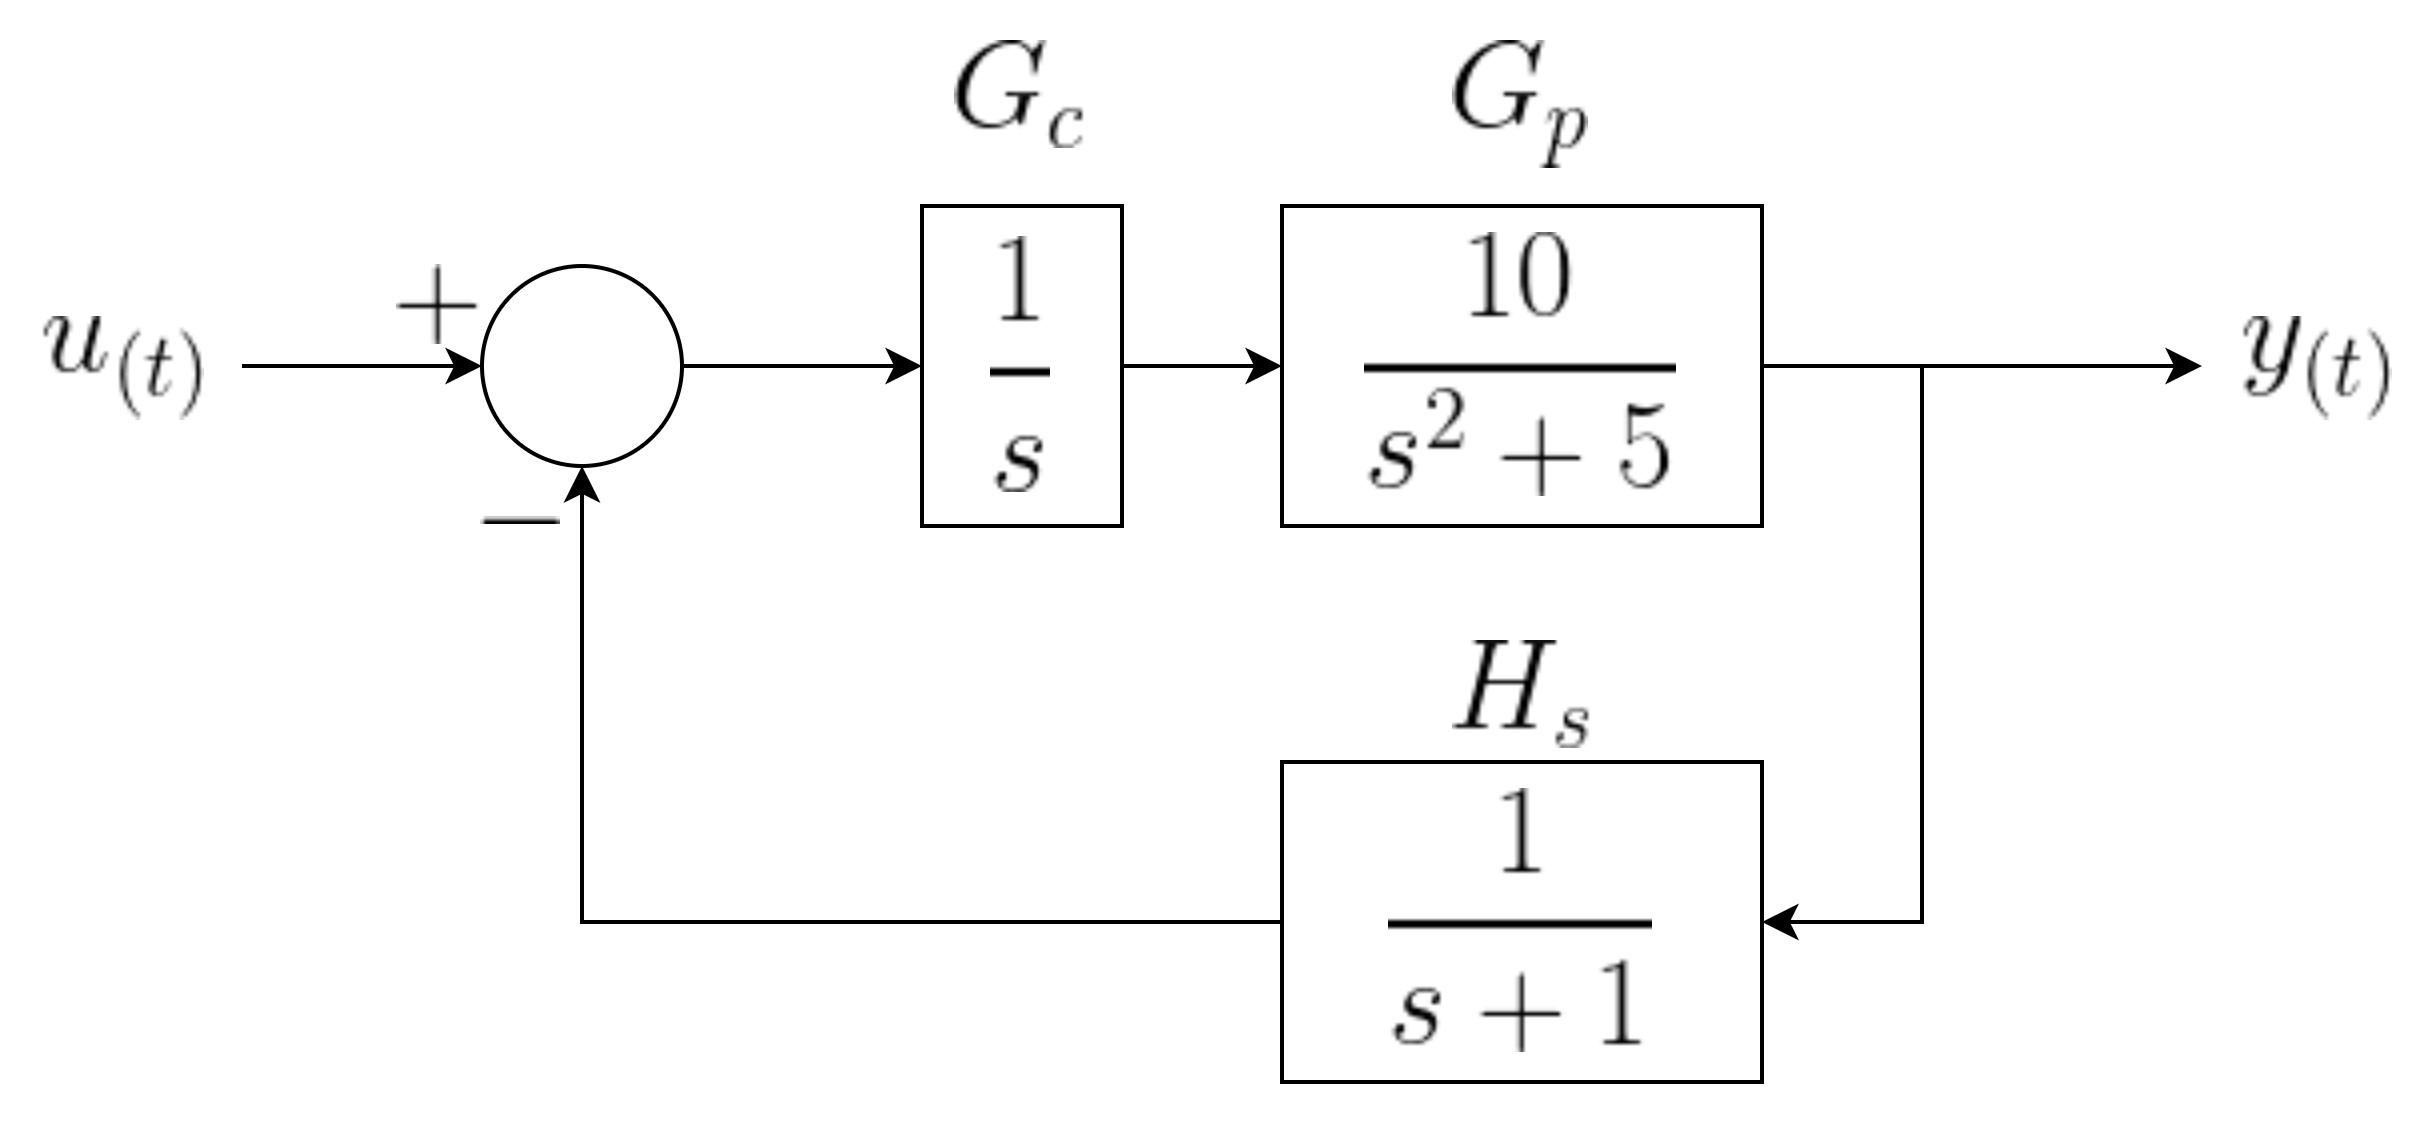
\includegraphics[width = 0.7\textwidth]{assets/image/blokDiagram.png}
                \caption{Diagram blok sistem}
                \label{gambar_1}
            \end{figure}
            \begin{equation}
                \begin{split}
                    G &= G_c    G_p \\[5pt]
                    G &= \frac{1}{s} \left(\frac{10}{s+5}\right) \\[5pt]
                    G &= \frac{10}{s^2+5s}
                    \label{persamaan_8}
                \end{split}
            \end{equation}
            Hasil penyederhanaan blok $G$ dapat dilihat pada blok diagram gambar \ref{gambar_2}.
            \begin{figure}[H]
                \centering
                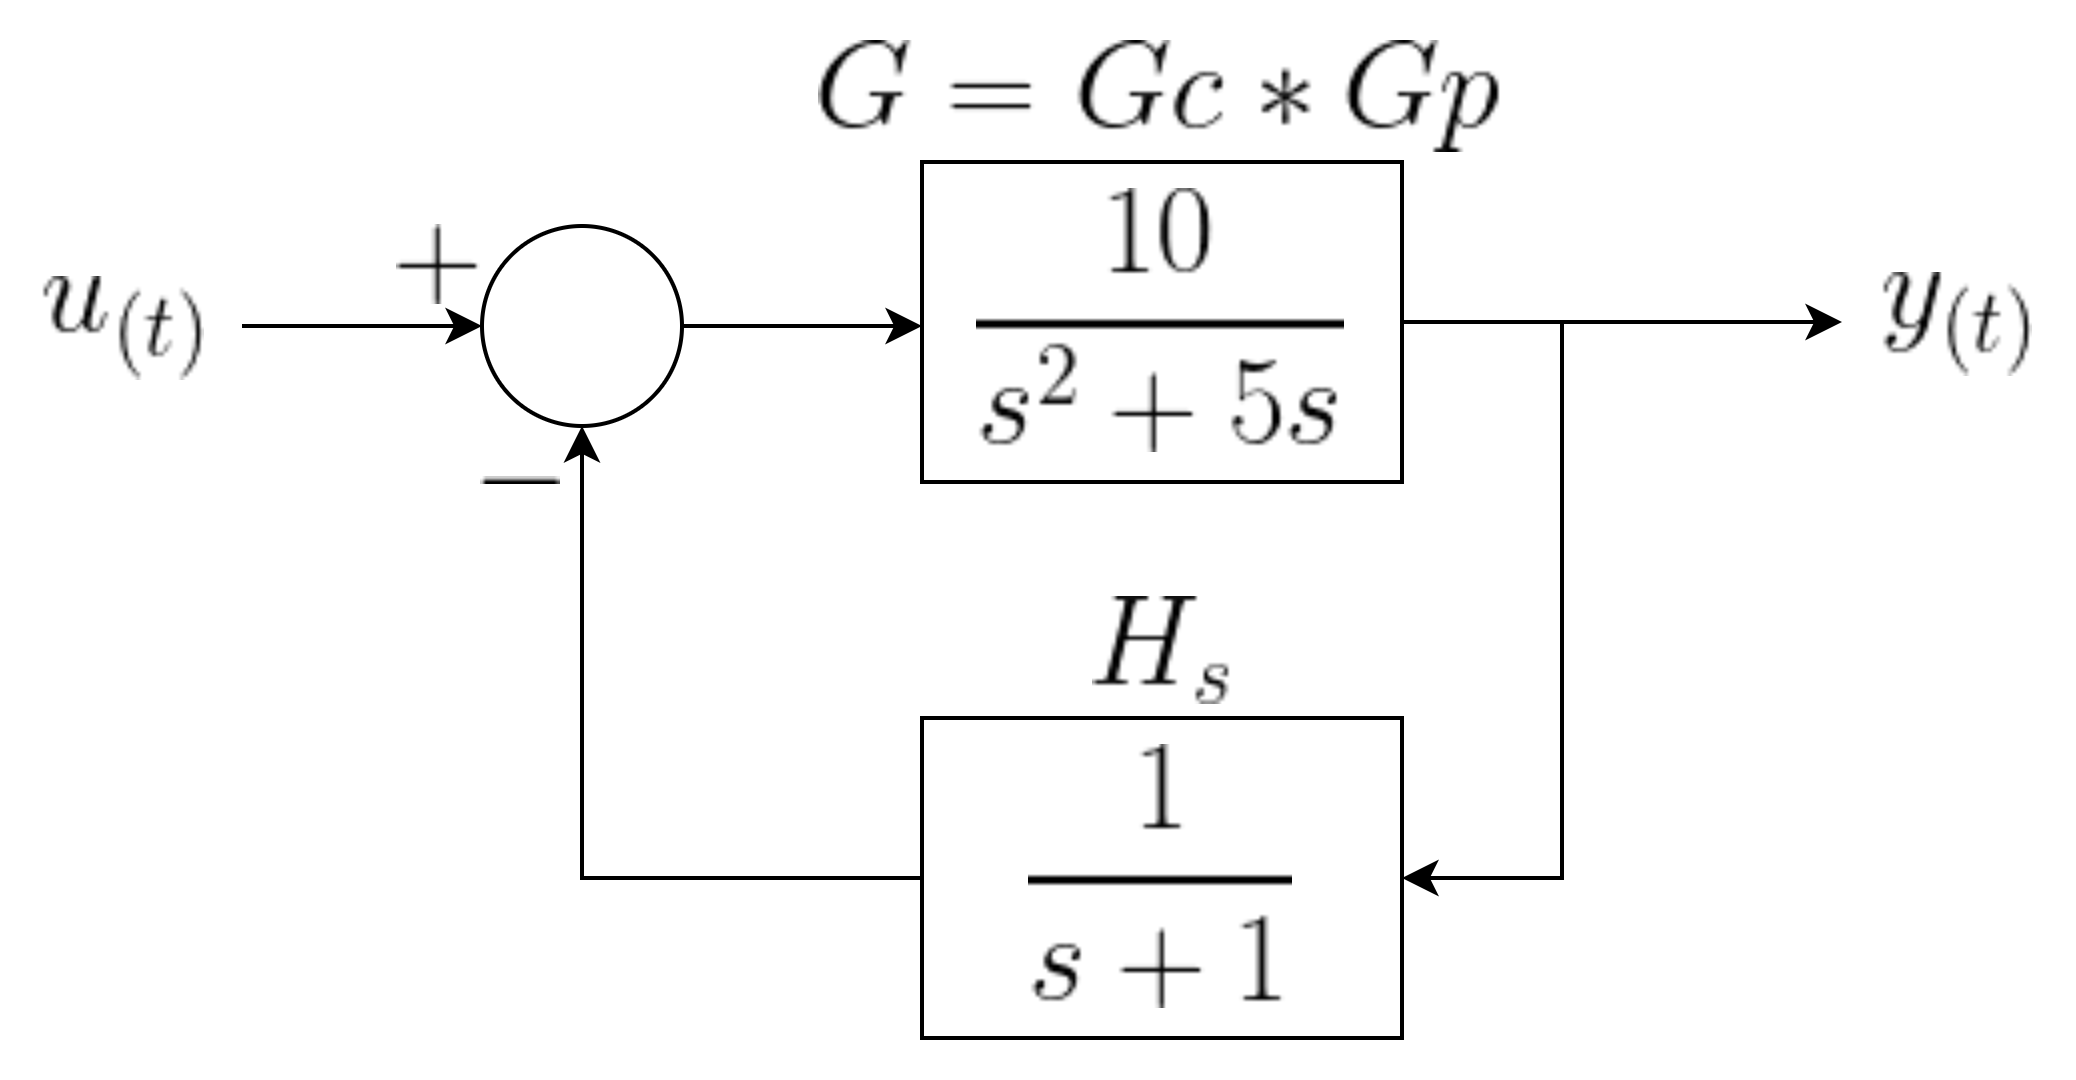
\includegraphics[width = 0.7\textwidth]{assets/image/blokDiagram_Simplified.png}
                \caption{Diagram blok sistem setelah disederhanakan}
                \label{gambar_2}
            \end{figure}
            Untuk medapatkan fungsi transfer sistem. blok dianalisis dengan persamaan \textit{feedback} sebagai berikut,
            \begin{equation}
                \begin{split}
                         \frac{y}{u} &= \frac{G}{1+GH_s} \\[5pt]
                                     &= \ffrac{\frac{10}{s^2+5s}}{1+(\frac{10}{s^2+5s}\frac{1}{s+1}} \\[5pt]
                                     &= \ffrac{\frac{10}{s^2+5s}}{\frac{(s^2+5s)  (s+1)}{(s^2+5s)  (s+1)}+\frac{10}{(s^2+5s)  (s+1)}} \\[5pt]
                                     &= \frac{10}{s^2+5s}    \frac{(s^2+5s)  (s+1)}{(s^2+5s)  (s+1) + 10} \\[5pt]
                                     &= \frac{10  (s+1)}{(s^2+5s)  (s+1) + 10}\\[5pt]
                         \frac{y}{u} &= \frac{10s+10}{s^3+6s^2+5s+10}
                         \label{persamaan_9}
                \end{split}
            \end{equation}
        \subsubsection{Mencari step respon dari blok prosess}
        $G_p$ merupakan sistem orde pertama, sehingga analisis sistem dilakukan menggunakan persamaan sebagai berikut,
            \begin{equation}
                \frac{R}{C} = \frac{K}{\tau s + 1} \\[5pt]
                \label{persamaan_16}
            \end{equation}
            Mengacu pada persamaan \eqref{persamaan_16}, maka blok proses dapat dianalisa sebagai berikut,
            \begin{equation}
                \begin{split}
                    \frac{R}{C} &= \frac{10}{s+5} \rightarrow \frac{K}{\tau s + 1} \\[5pt]
                                &= \ffrac{\frac{10}{5}}{\frac{1}{5}s + \frac{5}{5}} \\[5pt]
                                &= \frac{2}{0.2s + 1}
                \label{persamaan_17}
                \end{split}
            \end{equation}
            Dari persamaan \eqref{persamaan_17} dapat diketahui nilai $K = 2$ dan nilai $\tau = 0.2$. Dari nilai-nilai tersebut dapat dibuat plot dengan MATLAB sebagai berikut,
            \begin{figure}[H]
                \centering
                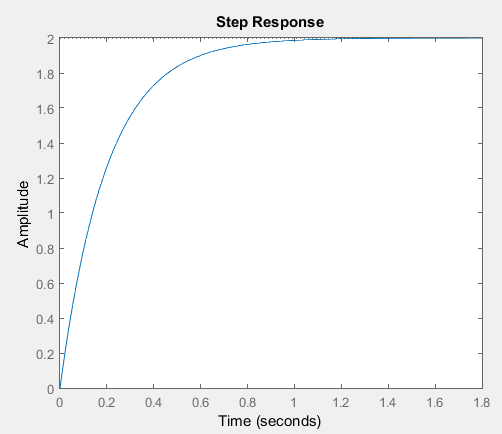
\includegraphics[width = 0.7\textwidth]{assets/image/plotStepSys.png}
                \caption{Hasil step sistem dengan MATLAB}
                \label{gambar_3}
            \end{figure}
        \subsubsection{Mencari persamaan state-space}
            \begin{equation}
                \begin{split}
                    \frac{y}{u} &= \frac{10s+10}{s^3+6s^2+5s+10} \\[5pt]
                    \frac{y}{u} &= \underbrace{\frac{1}{s^3+6s^2+5s+10}}_\text{mencari persamaan $\dot{x}=Ax+Bu$} \overbrace{(10s+10)}^\text{mencari persamaan $y=Cx+Du$}
                    \label{persamaan_10}
                \end{split}
            \end{equation}
            Dari persamaan \eqref{persamaan_10} dapat dicari persamaan \textit{input state-space} sebagai berikut,
            \begin{equation}
                \begin{split}
                    \frac{y}{u} &= \frac{1}{s^3+6s^2+5s+10} \\[5pt]
                             1u &= (s^3+6s^2+5s+10)y \\[5pt]
                             1u &= \frac{dy^3}{dt^3} + 6\frac{dy^2}{dt^2} + 5\frac{dy}{dt} + 10y \\[5pt]
                             1u &= \dddot{y} + 6\ddot{y} + 5\dot{y} + 10y \\[5pt]
                       \dddot{y} &= -6\ddot{y} - 5\dot{y} - 10y + 1u
                       \label{persamaan_11}
                \end{split}
            \end{equation}
            Didapatkan aturan dari persamaan \eqref{persamaan_11} sebagai berikut,
            \begin{equation}
                \begin{split}
                    x_1 &= y \\[5pt]
                    x_2 &= \dot{x_1} = \dot{y} \\[5pt]
                    x_3 &= \dot{x_2} = \ddot{y}
                    \label{persamaan_12}
                \end{split}
            \end{equation}
            Persamaan \textit{input state-space} dapat dicari dari persamamaan \eqref{persamaan_11} dan aturan \eqref{persamaan_12} sebagai berikut,
            \begin{equation}
                \begin{split}
                    \dot{x} &= Ax+ Bu \\[10pt]
                    \begin{bmatrix} \dot{x_1} \\ \dot{x_2} \\ \dot{x_3} \end{bmatrix}&=\begin{bmatrix} 0 & 1 & 0 \\ 0 & 0 & 1 \\ -10 & -5 & -6\end{bmatrix} \begin{bmatrix} x_1 \\ x_2 \\x_3 \end{bmatrix} + \begin{bmatrix} 0 \\ 0 \\ 1 \end{bmatrix} u
                \label{persamaan_13}
                \end{split}
            \end{equation}
            persamaan \textit{output state-space} sistem dapat dicari dari persamaan \eqref{persamaan_10} sebagai berikut,
            \begin{equation}
                \begin{split}
                    \frac{y}{u} &= 10s+10 \\[5pt]
                              y &= (10s+10)u \\[5pt]
                              y &= 10\frac{du}{dt} + 10u
                              \label{persamaan_14}
                \end{split}
            \end{equation}
            Dari persamaan \eqref{persamaan_14} didapatkan aturan sebagai berikut,
            \begin{equation}
                \begin{split}
                    x_1 &= u \\[5pt]
                    x_2 &= \dot{x_1} = \dot{u} \\[5pt]
                    x_3 &= \dot{x_2} = \ddot{u}
                    \label{persamaan_15}
                \end{split}
            \end{equation}
            Persamaan output dapat dicari dari persamaan \eqref{persamaan_14} dan aturan \eqref{persamaan_15} sebagai berikut,
            \begin{equation}
                \begin{split}
                    y &= Cx + Du \\[5pt]
                    y &= \begin{bmatrix} 10 & 10 & 0\end{bmatrix} \begin{bmatrix} x_1 \\ x_2 \\ x_3 \end{bmatrix}
                \end{split}
            \end{equation}
            Hasil perhitungan dibandingkan dengan Matlab untuk memverifikasi kebenaran perhitungan \textit{state-space}. Kode MATLAB yang digunakan untuk konversi dari fungsi transfer ke \textit{state-space} sebagai berikut,
            \begin{figure}[H]
                \centering
                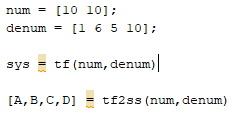
\includegraphics[width = 0.5\textwidth]{assets/image/kodeMatlab.png}
                \caption{Kode program untuk konversi fungsi transfer ke \textit{state-space}}
                \label{gambar_4}
            \end{figure}
            \begin{figure}[H]
                \centering
                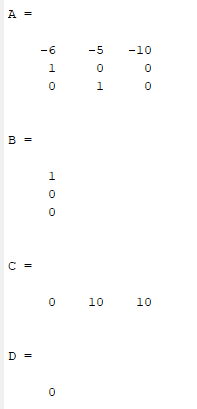
\includegraphics[width = 0.25\textwidth]{assets/image/outSSMatlab.png}
                \caption{Nilai state-space dari program yang dijalankan}
                \label{gambar_5}
            \end{figure}
            Dari perbandingan hasil perhitungan manual dengan perhitungan menggunakan program MATLAB memiliki nilai yang sama, hanya saja nilai polynomial pada program matlab dimulai dari nilai pangkat polynomial tertinggi sedangkan pada perhitungan manual nilai pangkat polynomial dimulai dari pangkat terendah. Sehingga, terdapat perbedaan tata letak nilai-nilai \textit{state-space}.
    \subsection{Latihan Soal 2}
        Pada soal ini, dilakukan analisis reprensentasi \textit{state-space} pada persamaan berikut,
        \begin{equation}
            \dddot{y} + 3\ddot{y} + 2\dot{y} = u
            \label{persamaan_18}
        \end{equation}
        Representasi dapat dilakukan dengan menetapkan aturan berdasarkan persamaan \eqref{persamaan_18} sebagai berikut,
        \begin{equation}
            \begin{split}
                x_1 &= y \\[5pt]
                x_2 &= \dot{x_1} = \dot{y} \\[5pt]
                x_3 &= \dot{x_2} = \ddot{y}
                \label{persamaan_19}
            \end{split}
        \end{equation}
        Persamaan \eqref{persamaan_18} dapat diubah untuk mencari nilai \textit{state-space} sebagai berikut,
        \begin{equation}
            \begin{split}
                \dddot{y} + 3\ddot{y} + 2\dot{y} = u \\[5pt]
                \dddot{y} = - 3\ddot{y} - 2\dot{y} + u \\[5pt]
                \label{persamaan_20}
            \end{split}
        \end{equation}
        Dari persamaan \eqref{persamaan_20} dan aturan \eqref{persamaan_19} dapat dibuat persamaan \textit{state-space} sebagai berikut,
        \begin{equation}
            \begin{split}
                \dot{x} &= Ax +Bu \\[5pt]
                \begin{bmatrix} x_1 \\ x_2 \\ x_3\end{bmatrix} &= \begin{bmatrix} 0 & 1 & 0 \\ 0 & 0 & 1 \\ 0 & -2 & -3 \end{bmatrix} \begin{bmatrix} x_1 \\ x_2 \\ x_3 \end{bmatrix} + \begin{bmatrix} 0 \\ 0 \\ 1 \end{bmatrix} u
                \label{persamaan_21}
            \end{split}
        \end{equation}
        Persamaan \textit{output} dapat ditulis sebagai berikut,
        \begin{equation}
            \begin{split}
                y = Cx + Du \\[5pt]
                y = \begin{bmatrix} 1 & 0 & 0 \end{bmatrix} \begin{bmatrix} x_1 \\ x_2 \\ x_3 \end{bmatrix}
            \end{split}
            \label{persamaan_22}
        \end{equation}
        Dari hasil analisis yang dilakukan ditemukan persamaan \textit{state-space} dan persamaan \textit{output} masing-masing pada persamaan \eqref{persamaan_21} dan persamaan \eqref{persamaan_22}.
\section{Kesimpulan}
    Kesimpulan yang dapat diperoleh dari praktikum ini antara lain,
    \begin{enumerate}
        \item Model state space dapat dikonversi dari fungsi alih maupun sebaliknya
        \item Urutan penulisan posisi pangkat state space dapat dilakukan dari polynomial yang terkecil ataupun yang terbesar
    \end{enumerate}
\begin{thebibliography}{2}
    \bibitem[1]{Fahmizal} Fahmizal. 2020. "Perkenalan State Space" dalam \textit{Modul Praktikum Teknik Kendali Lanjut} (hlm.1-10). Yogyakarta
\end{thebibliography}
    
\end{document}
